\documentclass[11pt, oneside]{article} 
\usepackage{geometry}
\geometry{letterpaper} 
\usepackage{graphicx}
	
\usepackage{amssymb}
\usepackage{amsmath}
\usepackage{parskip}
\usepackage{color}
\usepackage{hyperref}

\graphicspath{{/Users/telliott_admin/Dropbox/Tex/png/}}
% \begin{center} 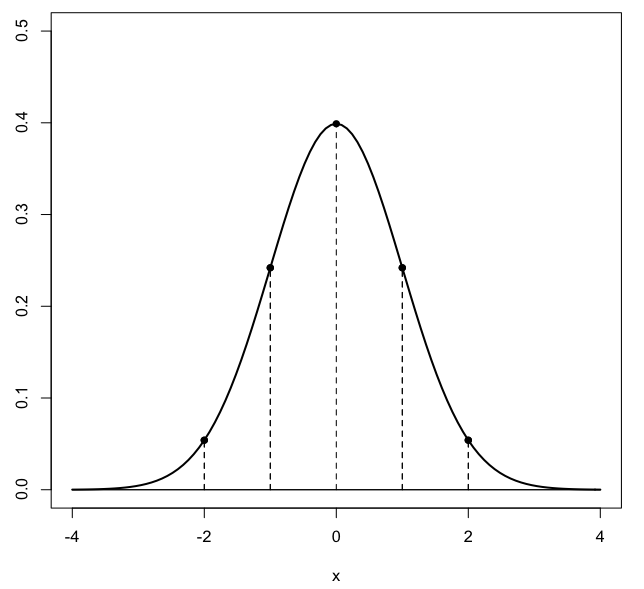
\includegraphics [scale=0.4] {gauss3.png} \end{center}

%break
\title{Expected value}
\date{}

\begin{document}
\maketitle
\Large

David Morin:
\begin{quote}\color{blue}Consider a variable that can take on certain numerical values with certain probabilities.  Such a variable is appropriately called a \emph{random variable}\color{black}\end{quote}

Examples:

$\circ$ A coin is tossed and the outcome is assigned $1$ (heads) or $0$ (tails).

$\circ$ A coin tossed twice; the outcome is assigned a number based on the total count of heads:  $0$ (TT), $1$ (HT,TH) or $2$ (HH).

$\circ$ A fair die is thrown;  the outcome is assigned the value facing up.

If we say that $X$ is a random variable that represents the outcomes in the example 3, and the values it can take on are
\[ x_1 = 1, x_2 = 2 \dots x_6 = 6 \]

The probabilities for the outcomes $x_1, x_2 \dots$ do not have to be equal.  In example 2, the probabilities are $p_1 = 0.25$, $p_2 = 0.5$ and $p_3 = 0.25$.

\begin{quote}\color{blue}The collection of these probabilities is the \emph{probability distribution} for $X$.\end{quote}

\begin{quote}The \emph{expectation value} or \emph{expected value} of a random variable $X$ is the expected average obtained in a large number of trials of the process (in trials yet to be carried out).\color{black}\end{quote}

$\bullet$ In a large number of trials each outcome $x_i$ will occur with probability $p_i$ and the expected value is
\[ E(X) = \sum_i p_i x_i  \]

The expected value $E(X)$ is often written $\mu_x$ or even just $\mu$ if the meaning is clear.  For example 3, the roll of a die, we have

\[ E = \sum_i p_i x_i = \frac{1}{6} \cdot 1 + \dots + \frac{1}{6} \cdot 6  \]
\[ = \frac{1}{6} \cdot (1 + 2 + 3 + 4 + 5 + 6 ) \]
\[ = \frac{21}{3} = 3.5 \]

Note that here $E(X)$ is not one of the values that $X$ can actually take on.

\begin{quote}\color{blue}You might think that the expected value is the value that is most likely to occur.  This is \emph{not} the case.\color{black}\end{quote}

$\circ$ Suppose you flip a coin 4 times ($H = 1, T = 0$).  Obviously the expected value is 2.  More explicitly, we use the combinations ("choose") formula to write

\[ E(X) = \frac{1}{16} \ 0 + \frac{4}{16} \ 1 + \frac{6}{16} \ 2 + \frac{4}{16} \ 3 + \frac{1}{16} \ 4 \]
\[ = \frac{1}{16} \ (0 + 4 + 12 + 12 + 4) \]
\[ = \frac{32}{16} = 2 \]

$\circ$ Flip a coin until heads is obtained.  Obviously, the expected value is 1, since we get all zeroes until the last flip, where we get 1. 

There is a probability of $1/2$ for heads on the first flip.  There is a probability of $1/2$ that we proceed to the second flip, times $P=1/2$ that we obtain heads on that one, for a total of $P = 1/4$ for heads on the second flip, and so on.

\[ E(X) = \frac{1}{2} \ 1 + \frac{1}{4} (0 + 1) +  \frac{1}{8}(0 + 0 + 1) + \dots = 1 \]

$\circ$ On the other hand, if we define $X$ instead as \emph{the total number of times the coin is flipped}, we have

\[ E(X) = \sum_{i=1}^{\infty} \frac{1}{2^i} \ i \]
\[ E(X) = \frac{1}{2} (1) + \frac{1}{4} (2) +  \frac{1}{8}(3) +  \frac{1}{16}(4) +  \frac{1}{32}(5) + \dots \]
\[ = \frac{1}{2} + \frac{2}{4} + \frac{3}{8} + \frac{4}{16} + \frac{5}{32} + \dots \]

This is not a series I remembered when working through this initially.  There is a trick which I saw in \emph{Grinstead and Snell}, and eventually I remembered another approach which I learned in \emph{Strang}. I'll show both below, but let's work with the series a bit.

The nth term in the series is $n/2^n$.  The ratio of successive terms is
\[ \frac{n+1}{2^{n+1}} \ \frac{2^n}{n} = \frac{n+1}{2n} \]
which approaches one-half as $n \rightarrow \infty$, so we know the series converges (absolutely).

Calculating the sum of the first ten terms:

\begin{verbatim}
1 0.5
2 1.0
3 1.375
4 1.625
5 1.78125
6 1.875
7 1.9296875
8 1.9609375
9 1.978515625
10 1.98828125
\end{verbatim}

With 20 terms the result is $1.999979$.  It's pretty clear that the result is 2.

For the analytical approach:
\[ E(X) = \sum_{i=1}^{\infty} \frac{1}{2^i} \ i = \ ? \]

Consider that the series without the factor of $i$ is just the geometric series with $r=1/2$ and initial value $1$ and its sum is:
\[ \sum_{i=1}^{\infty} \frac{1}{2^i} = \frac{1}{2} + \frac{1}{4} + \frac{1}{8} + \dots = 1 \]

Why not add up many copies of this series, starting each version from the \emph{succeeding index}:
\[ \sum_{i=1}^{\infty} \frac{1}{2^i} + \sum_{i=2}^{\infty} \frac{1}{2^i} + \sum_{i=3}^{\infty} \frac{1}{2^i} + \dots \]

The result will have $2$ occurrences of $1/2^2$ and $3$ of $1/2^3$ and so on.  I claim that:
\[ \sum_{i=1}^{\infty} i \ \frac{1}{2^i}  = \sum_{i=1}^{\infty} \frac{1}{2^i} + \sum_{i=2}^{\infty} \frac{1}{2^i} + \sum_{i=3}^{\infty} \frac{1}{2^i} + \dots \]

Now, the first term adds up to $1$, the second adds up to $1 - 1/2 = 1/2$ (since the first term is missing), the third to $1 - 3/4 = 1/4$ (since the first two terms are missing) and so on giving
\[ 1 + \frac{1}{2} + \frac{1}{4} + \dots = 2 \]
In other words
\[ \sum_{i=1}^{\infty} i \ \frac{1}{2^i} = \sum_{i=0}^{\infty} \ \frac{1}{2^i} \]
which is rather surprising.

For another approach to the analysis, start with this equality
\[ 1 + x + x^2 + x^3 + \dots =  \frac{1}{1-x} \]
The formal proof looks at the partial sums as their number increases, but simply multiplying shows that:
\[ (1-x) (1 + x + x^2 + x^3 + \dots) \stackrel{?}{=} \]

Multiplying by $1$ just gives us the same series.  Multiplying by -x gives:
\[ -x - x^2 - x^3  + \dots \]
It's clear that every term after the first will cancel, so the sum is just $1$, as required.  

Now, the trick is to differentiate:
\[ \frac{d}{dx} \ 1 + x + x^2 + x^3  + x^4 + \dots = \frac{d}{dx} \ \frac{1}{1-x} \]
The left-hand side is
\[ 1 + 2x + 3x^2 + 4x^3 + \dots \]
This is \emph{almost} our series (with $x = 1/2$):
\[ \sum_{i=1}^{\infty} i \ \frac{1}{2^i} = \frac{1}{2} +  \frac{2}{2^2} +  \frac{3}{2^3}  + \dots \]
To obtain the exact series we must subtract the following (again, with $x = 1/2$)
\[ 1 + x + x^2 + x^3 + \dots = \sum_{i=0}^{\infty} \frac{1}{2^i} = 2 \]
Differentiating the other part we obtain
\[ \frac{d}{dx} \ \frac{1}{1-x} = \frac{1}{(1-x)^2} \]
(canceling the minus sign from the power and the one from the chain rule).

But as we said, $ x= 1/2$ so this part of the sum is equal to
\[ \frac{1}{(1-1/2)^2} = 4 \]
we have to subtract the other part, which was equal to $2$, yielding the final answer.

\subsection*{addition and multiplication of expectation}
$\bullet$ Addition rule for expected value (mean).
\[ E(X + Y) = E(X) + E(Y) \]
Proof:

In calculating $E(X + Y)$ we look at each value $x_i$ and associated probability $p_i$, and also at each value $y_j$ and its associated probability $q_j$.

The joint probability for both $x_i$ and $y_j$ being observed is $p_i q_j$ and the value of $X + Y$ is $x_i + y_j$ so the expected value is
\[ E(X + Y) = \sum_i \sum_j p_i q_j (x_i + y_j) \]

Now, breaking up the outer sum, we have for each $x_i$
\[ \sum_j p_i q_j (x_i + y_j) =  \sum_j p_i q_j x_i  +  \sum_j p_i q_j y_j \]
Both $x_i$ and $p_i$ are constants for each inner sum.

The first term on the right-hand side is
\[  \sum_j p_i q_j x_i = p_i  x_i \sum_j q_j = p_i x_i \]
while the second term is
\[ \sum_j p_i q_j y_j = p_i \sum_j q_j y_j = p_i E(Y) \]
Going back to the outer sum, we have then
\[ E(X + Y) = \sum_i p_i x_i + \sum_i  p_i E(Y) \]
\[ = \sum_i p_i x_i + E(Y) \sum_i  p_i \]
\[ = E(X) + E(Y) \]
$\square$

This does \emph{not} depend on $X$ and $Y$ being independent.

$\circ$ $X$ is a fair die and $Y$ a tossed coin.  We know that 
\[ E(X) = 3.5 \] 
\[ E(Y) = 0.5 \]
All cases have
\[ P = \frac{1}{6} \cdot \frac{1}{2} = \frac{1}{12} \]

Enumerating the cases for $X + Y$
\[ X = 0, \ \ Y = 1 \dots \ \  X = 0, \ \ Y = 6 \]
\[ X = 1, \ \ Y = 1 \dots \ \  X = 1, \ \ Y = 6 \]
The term $x_i + y_i$ summed over all of these cases is 
\[ (0 + 1) + (0 + 2) + \dots + (0 + 2) + (1 + 1) + (1 + 2) + \dots + (1 + 6) \]
\[ = 21 + 6 + 21 = 48 \]
We must divide by $12$ giving $4.0$.

$\bullet$ The general case for addition (with multiplication by a constant) is
\[ E(aX + bY + c) = aE(X) + bE(Y) + c \]
for constants $a$, $b$ and $c$.

$\bullet$ If we have $n$ random variables all associated with the same probability distribution, then
\[ E(X_1 + X_2 + \dots X_n) = E(X_1) + E(X_2) + \dots E(X_n) \]
\[ = n E(X) \]

$\circ$ Consider the permutations of $abc$.  There are six:
\[ abc, \ acb, \ bac, \ bca, \ cab, \ cba \]
Now, define the value of each permutation as the number of letters which lie in the same positions as they do in $abc$.  Namely
\[ abc = 3, \  acb = 1, \  bac = 1, \  bca = 0, \  cab = 0, \  cba = 1 \]

Let $X$ be a random variable which takes on this value when each of the permutations  (called the number of "fixed points") is obtained randomly.  
\begin{center} 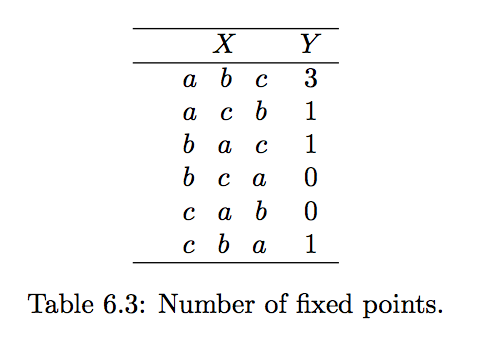
\includegraphics [scale=0.5] {fixed_points.png} \end{center}

What is the expected value of $X$?
\[ E(X) = \frac{1}{6} \ (3 + 1 + 1 + 0 + 0 + 1) = 1 \]

Now, we can use the addition rule to generalize this to the case where we have the set $\{1,2,3 \dots n\}$, and cannot simply enumerate the cases.  \emph{Grinstead and Snell}:

\begin{quote}\color{blue}Let $Z$ denote the random permutation. For each $i$, $1 \le i \le n$, let $X_i$ equal $1$ if $Z$ fixes $i$, and $0$ otherwise. So if we let $F$ denote the number of fixed points in $Z$, then\color{black}\end{quote}
\[ F = X_1 + X_2 + \dots + X_n \]

By the rule:
\[ E(F) = E(X_1) + E(X_2) + \dots + E(X_n) \]

\begin{quote}\color{blue}But it is easy to see that for each $i$\color{black}\end{quote}
\[ E(X_i) = \frac{1}{n} \]
so
\[ E(F) = 1 \]

$\bullet$ Multiplication rule for expected value (mean).
\[ E(X \cdot Y) = E(X) \cdot E(Y) \]
\emph{provided} $X$ and $Y$ are \emph{independent}.

Proof:
\[ E(X) \cdot E(Y) = \sum_i \sum_j p_i q_j (x_i \cdot y_j) \]
And again, for each $x_i$ the inner sum has constant $p_i$ and constant $x_i$ so we can write
\[ \sum_j p_i q_j (x_i \cdot y_j) = p_i x_i  \sum_j q_j (y_j) = p_i x_i E(Y) \]

Then, provided that $q_j$, the probability distribution for $Y$, does not depend on which $x$ we are considering, the various $E(Y)$ are all the same and the outer sum is
\[ \sum_i p_i x_i E(Y) \]
and since $E(Y)$ is constant 
\[ \sum_i p_i x_i E(Y) = E(Y)  \sum_i p_i x_i  = E(X) \cdot E(Y) \]
$\square$

Note that this equation is not valid:
\[ E(X) \cdot E(X) \stackrel{?}{=} E(X^2) \]
since the probability distribution for $X$ \emph{does} depend on $X$

$\circ$ Consider two dice.  If we roll them independently then:
\[ E(X + Y) = \frac{1}{36} (1 \cdot 2 + 2 \cdot 3 + 3 \cdot 4 + 4 \cdot 5 + 5 \cdot 6 \dots \]
\[ + \ 6 \cdot 7 + 5 \cdot 8 + 4 \cdot 9 + 3 \cdot 10 + 2 \cdot 11 + 1 \cdot 12) \]
\[ =  \frac{1}{36} (2 + 6 + 12 + 20 + 30 + 42 + 40 + 36 + 30 + 22 + 12) \]
\[ = \frac{1}{36} \ 252 = 7.0 \]
\[ = E(X) + E(Y) \]

$\circ$ But if we roll one die and then simply turn the other one so as to have the \emph{next} number up (e.g. $1$ is paired with $2$, $2$ with $3$, and so on, wrapping around so that $6$ is paired with $1$), we obtain
\[ E(X + Y) = \frac{1}{6} \ (3 + 5 + 7 + 9 + 11 + 1) \] 
\[ \frac{36}{6} \ne 7 \]

$\circ$ And if we roll one die and then simply turn the other one so as to have the \emph{same} number up, we obtain
\[ E(X + Y) = \frac{1}{6} \ (2 + 4 + 6 + 8 + 10 + 12) \] 
\[ \frac{42}{6} = 7 \]

For dependent variables $E(X+Y)$ depends on the probability distributions of the variables.

\subsection*{Variance}
$\bullet$ Variance is defined as:
\[ \text{Var}(X) = E[(X - \mu)^2 ] \]
where $\mu = E(X)$.  So
\[ \text{Var}(X) = \sum_i p_i (X_i - \mu)^2 \]

$\circ$ For throwing a fair die, we found that $E(X) = \mu = 3.5$.  The variance is:
\[ \text{Var}(X) = \frac{1}{6} \ (2.5^2 + 1.5^2 + 0.5^2 + 0.5^2 + 1.5^2 + 2.5^2) \]
\[ = \frac{1}{6} \ (2) (8.75) = 2.916 \]

$\circ$ For a coin flip, we found that $E(x) = \mu = 0.5$ 
\[ \text{Var}(X) = \frac{1}{2} \ [ \ (0-0.5)^2 + (1-0.5)^2 \ ] \  = 0.25 \]

$\circ$ For a biased coin that gives heads with frequency $p$, we found that
\[ E(X) = p \cdot 1 + (1-p) \cdot 0 = p \]
so
\[ \text{Var}(X) = p (1-p)^2 + (1-p)(0 - p)^2 \]
\[ = p(1-p) \ [ \ (1-p) + p \ ] \]
\[ = p(1-p) = pq \]

$\bullet$ Multiplication by a constant gives a factor of the constant squared in the variance.
\[ \text{Var}(aX) = a^2 \ \text{Var}(X) \]
Proof:
\[ E(aX) = aE(X) \]
so
\[ \text{Var}(aX) = \sum_i p_i (ax_i - a \mu)^2 \]
\[ = a^2  \sum_i p_i (x_i - \mu)^2 \]
\[ = a^2 \ \text{Var}(X) \]
$\square$

$\circ$ Suppose each dice roll's value is multiplied by a factor of 2.  Then
\[ E(X) = \frac{1}{6} \ (2 + 4 + 6 + 8 + 10 + 12) = 7 \]
\[ E \ [ \ (X - \mu)^2 \ ] \ = \frac{1}{6} \ [ \  (-5)^2 + (-3)^2 + (-1)^2 + 1^2 + 3^2 + 5^2) \ ]  \]
\[ = \frac{1}{6} (70) = 11.66 \approx 2^2 \cdot 2.92 \]

$\bullet$ Variances add.  This result is central to probability and statistics and it's the main point of this write-up.

\[ \text{Var}(X) + \text{Var}(Y) = \text{Var}(X + Y) \]

Proof:
\[ \text{Var}(X + Y) = E \ [ \ ((X + Y) - (\mu_{x + y}) )^2  \ ]  \]
Since expected values add, we can write 
\[ \mu_{x+y} = E(X+Y) = E(X) + E(Y) = \mu_x + \mu_y \]
so we can write
\[ \text{Var}(X + Y) = E \ [ \ ((X + Y) - (\mu_x + \mu_y) )^2  \ ]  \]
Rearrangement gives
\[ = E \ [ \ ((X - \mu_x) + (Y - \mu_y) )^2  \ ]  \]
Now, we just multiply out
\[ = E \ [ \ (X - \mu_x)^2 + 2( X - \mu_x) (Y - \mu_y) + (Y - \mu_y)^2  \ ]  \]
By the addition rule for expected values, we can break this up into three pieces:
\[ = E \ [ \ (X - \mu_x)^2 \ ] \ + E \ [ \ 2( X - \mu_x) (Y - \mu_y) \ ] \ + E \ [ \ (Y - \mu_y)^2  \ ]  \]
We will show that the middle term is zero.  What remains is the required result.
\[ = E \ [ \ (X - \mu_x)^2 \ ] \ + E \ [ \ (Y - \mu_y)^2  \ ]  \]
\[ = \text{Var}(X) + \text{Var}(Y) \]

To show that the middle term is zero, leave aside the factor of $2$ (using the multiplication rule) and we have:
\[ E \ [ \ (X - \mu_x) (Y - \mu_y) \ ] \]
By the multiplication rule for expected values (allowed since we said that $X$ and $Y$ are independent)
\[ = E(X - \mu_x) \cdot E(Y - \mu_y) \]
But 
\[ E(X - \mu_x) = E(X) - \mu_x \]
\[= \mu_x - \mu_x = 0 \]
so finally
\[ E \ [ \ (X - \mu_x) (Y - \mu_y) \ ] = 0 \]
$\square$

In fact, if $X$ and $Y$ are not independent, this term is the \emph{covariance}.

$\bullet$ Variances add but they don't multiply.

$\bullet$ Repeated sampling from the same distribution

If all of the $X_i$ are \emph{independent and identically distributed} (i.i.d.) variables, then
\[ = \text{Var}(X_1 + X_2 + \dots  + X_n) = n \text{Var}(X) \]

$\circ$ For a biased coin that gives heads with frequency $p$, we found that
\[ E(X) = p \cdot 1 + (1-p) \cdot 0 = p \]
and
\[ \text{Var}(X) = pq \]

For $n$ repeated trials with the same coin, the variance will be $npq$.

$\bullet$ An alternative form of the definition for variance can be derived pretty easily.  Start with the original form
\[ \text{Var}(X) = E \ [ (X - \mu)^2 \ ] \]
Multiply out:
\[ = E \ [ X^2 - 2 X \mu + \mu^2 \ ] \]
Use the addition rule for expected values:
\[ = E(X^2) - E(2 X \mu) + \mu^2 \ ] \]

But by the multiplication rule:
\[ E(2 X \mu) = 2 \mu E(X) = 2 \mu^2 \]
Hence
\[ E \ [ (X - \mu)^2 \ ] = E(X^2) - (E(x))^2 \]
\[ =  E(X^2) - \mu^2 \]
$\square$

$\circ$ Recall that the variance for rolls of a standard die is 2.9166.  The expected value is
\[ E(X) = \mu = 3.5 \]
\[ \mu^2 = 12.25 \]
And
\[ E(X^2) = \frac{1}{6} \ (1 + 4 + 9 + 16 + 25 + 36) \]
\[ = \frac{91}{6} = 15.1666 \]
And indeed
\[ 2.9166 = 15.1666 - 12.25 \]
The second version is usually preferred for calculation since it only does the subtraction once.
\[ \text{Var}(X) = E(X^2) - \mu^2 \]

\subsection*{Standard deviation}
The standard deviation is defined to be the square root of the variance.

$\bullet$ Since Var$(aX)$ = $a^2$ Var$(X)$:
\[  \text{SD}(aX) = a \cdot \text{SD}(X) \]

$\bullet$ The addition rule for variance can be written as
\[ \sigma_X^2 + \sigma_Y^2 = \sigma_{X+Y}^2\]

and it can be generalized as:
\[ {\sigma_{X1}}^2 + {\sigma_{X2}}^2 + \dots = {\sigma_{X_1 + X_2 + \dots}}^2 \]
\[ \sqrt{{\sigma_{X1}}^2 + {\sigma_{X2}}^2 + \dots} = \sigma_{X_1 + X_2 + \dots} \]

$\bullet$ If all of the $X_i$ are \emph{independent and identically distributed} random variables, then this result becomes
\[ \sigma_{X_1 + X_2 + \dots} = \sqrt{n {\sigma_{X}}^2} = \sqrt{n} \sigma_{X}  \]

$\circ$ Recall that the variance for a process with odds of success $p$ is
\[ \text{Var} \ (X) = np(1-p) = npq \]

The standard deviation is $\sqrt{npq}$.  For a fair coin, 
\[ \sqrt{pq} = \frac{1}{2} \]

The standard deviation of the number of Heads in $n = 100$ fair coin flips is 5 and in $n=10,000$ flips it is 50.

Suppose you roll a die $10,000$ times.  How many of those rolls should yield a $6$?

This is equivalent to a process with $p = 0.16$.  According to the formulas we've seen
\[ E(X) = p = 0.16 \]
 for one roll and
\[ E(X) = np = 1667 \]
for all the rolls roll together.  The standard deviation is:
\[ SD(X) = \sqrt{npq} = 37\]
So three standard deviations is $111$ and you are \emph{extremely} unlikely to observe a result outside the range $1667 \pm 111$.  (There are 3 chances in 1000 of this happening).

$\bullet$ Recall the alternative formula for the variance
\[ \text{Var} \ (X) = E(X^2) - \mu^2 = \sigma^2 \]
Thus
\[ E(X^2) = \sigma^2 + \mu^2 \]
and if the mean is zero then
\[ E(X^2) = \sigma^2  \]

 \subsection*{Standard error}
 The standard error of the mean relates to the variance or standard deviation for a series of values taken from some unknown probability distribution.
 
 Suppose we let $\bar{x}$ equal to the mean of a particular draw (say, $n$ values).  We now ask, what is
\[ \text{Var}(\bar{X}) = \ \ ? \]
By definition
\[ \bar{X} = \frac{X_1 + X_2 + \dots + X_n}{n} \]
so
\[ \text{Var}(\bar{X}) = \text{Var}( \frac{X_1 + X_2 + \dots + X_n}{n}) \]

Recall that multiplication by a constant gives a factor of the constant squared in the variance.
\[ = \frac{1}{n^2} \text{Var}(X_1 + X_2 + \dots + X_n) \]
\[ = \frac{1}{n^2} \text{Var}(n X) \]
\[ = \frac{1}{n} \text{Var}(X) \]
So the standard deviation of $\bar{x}$ is equal to the standard deviation of $X$ divided by the square root of $n$.

If we draw repeatedly and calculate $\bar{X}$ as a random variable, it will have a standard deviation that is smaller than the standard deviation of $X$ itself by a factor of $\sqrt{n}$.

$\bullet$ A major result from this discussion is that variances are additive.  I found this article on the web

\url{http://apcentral.collegeboard.com/apc/members/courses/teachers_corner/50250.html}

which calls this result the Pythagorean Theorem of statistics:
\[ SD^2(X \pm Y) = SD^2(X) + SD^2(Y) \]

\begin{quote}\color{blue}Just as the Pythagorean theorem applies only to right triangles, this relationship applies only to independent random variables.\color{black}\end{quote}

What's nice about this formulation is that it makes it easy to remember that the relationship is true only for \emph{independent} random variables.  The article has a great counter-example:

\begin{quote}\color{blue}Consider a survey in which we ask people two questions: During the last 24 hours, how many hours were you asleep? And how many hours were you awake?

There will be some mean number of sleeping hours for the group, with some standard deviation. There will also be a mean and standard deviation of waking hours. But now let's sum the two answers for each person. What's the standard deviation of this sum? It's 0, because that sum is 24 hours for everyone -- a constant. Clearly variances did not add here.\color{black}\end{quote}

\end{document} 